\documentclass[tikz, border=10pt]{standalone}
\usepackage{tikz}
\usepackage{amsmath, amssymb}
\usepackage{graphicx}
\usetikzlibrary{arrows.meta, fit, shapes.geometric, backgrounds, calc}

\definecolor{Blue}{HTML}{1F3A6E}
\definecolor{Red}{HTML}{8B1A1A}
\definecolor{Grn}{HTML}{1A5230}
\definecolor{Ink}{HTML}{1C1C1C}

% ─── Icon draw commands (all draw relative to origin) ───────────────────────

% Globe, radius r
\newcommand{\drawglobe}[2][Blue]{%
  \draw[#1,lw=0.55pt,fill=#1!7](0,0)circle(#2);
  \draw[#1,lw=0.32pt](-#2,0)arc(180:0:#2 and {0.36*#2});
  \draw[#1,lw=0.32pt,dashed](-#2,0)arc(180:360:#2 and {0.36*#2});
  \draw[#1,lw=0.32pt](0,-#2)--(0,#2);
  \draw[#1,lw=0.32pt]({-0.86*#2},{-0.5*#2})--({0.86*#2},{-0.5*#2});
  \draw[#1,lw=0.32pt]({-0.86*#2},{ 0.5*#2})--({0.86*#2},{ 0.5*#2});
}

% Person silhouette
\newcommand{\drawperson}[1][Blue]{%
  \draw[#1,fill=#1!25,lw=0.5pt](0,0.29cm)circle(0.11cm);
  \draw[#1,fill=#1!12,lw=0.45pt,rounded corners=1.2pt]
    (-0.13cm,0.16cm)rectangle(0.13cm,-0.16cm);
  \draw[#1,lw=0.45pt](-0.13cm,0.07cm)--(-0.23cm,-0.06cm);
  \draw[#1,lw=0.45pt]( 0.13cm,0.07cm)--( 0.23cm,-0.06cm);
  \draw[#1,lw=0.45pt](-0.06cm,-0.16cm)--(-0.09cm,-0.30cm);
  \draw[#1,lw=0.45pt]( 0.06cm,-0.16cm)--( 0.09cm,-0.30cm);
}

% Gear
\newcommand{\drawgear}[3][Red]{%
  \foreach \a in {0,40,80,120,160,200,240,280,320}{
    \draw[#1,fill=#1!12,lw=0pt](\a:#2)--({\a+18}:#2)--({\a+18}:{#2*1.38})--(\a:{#2*1.38})--cycle;}
  \draw[#1,fill=#1!10,lw=0.6pt](0,0)circle(#2);
  \draw[#1,fill=white,lw=0pt](0,0)circle(#3);
  \draw[#1,lw=0.5pt](0,0)circle(#3);
}

% Neural net 3-2-3
\newcommand{\drawnet}[1][Blue]{%
  \foreach \y in {-0.18cm,0cm,0.18cm}{
    \draw[#1,fill=#1!18,lw=0.35pt](-0.25cm,\y)circle(0.055cm);
    \draw[#1,fill=#1!18,lw=0.35pt]( 0.25cm,\y)circle(0.055cm);}
  \foreach \y in {-0.09cm,0.09cm}{\draw[#1,fill=#1!32,lw=0.35pt](0cm,\y)circle(0.065cm);}
  \foreach \yl in {-0.18cm,0cm,0.18cm}
    \foreach \yh in {-0.09cm,0.09cm}{
      \draw[#1!38,lw=0.24pt](-0.195cm,\yl)--(-0.065cm,\yh);
      \draw[#1!38,lw=0.24pt]( 0.065cm,\yh)--( 0.195cm,\yl);}
}

% ─── Global line-width shortcut ─────────────────────────────────────────────
\tikzset{lw/.style={line width=#1}}

\tikzset{
  blk/.style={draw=#1,fill=#1!7,rounded corners=3.5pt,lw=0.95pt,
    inner xsep=10pt,inner ysep=6pt,minimum width=6.2cm,
    text centered,font=\small\bfseries\sffamily,text=Ink},
  chip/.style={draw=Blue!55,fill=Blue!8,rounded corners=2.5pt,
    lw=0.75pt,inner xsep=5pt,inner ysep=4pt,
    minimum width=1.28cm,minimum height=0.72cm,
    text centered,font=\scriptsize\bfseries\sffamily,text=Ink},
  mppiblk/.style={draw=Red,fill=Red!7,rounded corners=3pt,lw=0.85pt,
    inner xsep=7pt,inner ysep=5pt,minimum width=3.20cm,minimum height=0.55cm,
    text centered,font=\footnotesize\bfseries\sffamily,text=Ink},
  A/.style ={-{Stealth[length=4.8pt,width=3.8pt]},lw=0.85pt,color=Ink!75},
  Ar/.style={-{Stealth[length=4.8pt,width=3.8pt]},lw=0.85pt,color=Red},
  Ag/.style={-{Stealth[length=4.8pt,width=3.8pt]},lw=0.85pt,color=Grn},
  panel/.style={draw=#1!35,fill=#1!4,rounded corners=5pt,lw=0.75pt,dashed,inner sep=8pt},
  % badge: small filled circle for icon at box corner
  badge/.style={circle,fill=#1!10,draw=#1!50,lw=0.55pt,
    minimum size=0.54cm,inner sep=0pt},
}

\begin{document}
\begin{tikzpicture}

%% ===================================================================
%%  Icons strategy:
%%  - Inline \tikz{} in LABEL-ONLY nodes (WVS label, MPPI label)
%%  - Badge nodes at NW corner of LLM + Cultural Alignment boxes
%%  - Debate scene drawn freely inside persona container
%%  All box TEXT nodes are PLAIN — no phantom hacks.
%% ===================================================================

%── (1) INPUT ─────────────────────────────────────────────────────────
\node[blk=Blue,minimum height=0.68cm](IN) at (0,0)
  {\raisebox{-0.12cm}{
\includegraphics[width=0.45cm]{icons/moral_scale.png}}\enspace Moral Scenario + Country $c$};

%── (2) PERSONA CONTAINER ─────────────────────────────────────────────
\node[draw=Blue!45,fill=Blue!4,rounded corners=3pt,lw=0.80pt,
      dashed,minimum width=6.2cm,minimum height=1.95cm]
  (PB) at (0,-1.625){};

% WVS label with inline globe icon
\node[font=\scriptsize\bfseries\sffamily,text=Blue,anchor=north]
  at (0,-0.74) {%
  \raisebox{-0.08cm}{
\includegraphics[width=0.35cm]{icons/culture_globe.png}}%
  \enspace WVS-Grounded Persona Panel ($N\!=\!4$)};

% Debate scene: 4 person silhouettes + speech arrows
\foreach \xp in {-1.85cm,-0.62cm,0.62cm,1.85cm}{
  \begin{scope}[shift={(\xp,-1.46cm)}]\drawperson[Blue]\end{scope}}
\foreach \xa/\xb in {-1.52cm/-0.95cm,-0.29cm/0.29cm,0.95cm/1.52cm}{
  \draw[Blue!50,
    {Stealth[length=3pt,width=2.4pt]}-{Stealth[length=3pt,width=2.4pt]},
    lw=0.48pt](\xa,-1.46cm)--(\xb,-1.46cm);}

% Persona chips
\foreach \i/\t in {1/Young,2/Mid-age,3/Elder,4/Utilit.}{
  \node[chip](P\i) at ({(\i-2.5)*1.55cm},-2.06cm){$P_{\i}$~~\t};}

%── (3) LLM ───────────────────────────────────────────────────────────
\node[blk=Blue,minimum height=0.84cm](LLM) at (0,-2.88)
  {Shared LLM Forward Pass\\[1pt]
   {\footnotesize\normalfont\mdseries
    base prefix $+$ $N$ persona prefixes in parallel}};

% Neural-net badge at NW corner of LLM
\node[inner sep=0pt] (LLMB) at ($(LLM.west)+(0,0)$){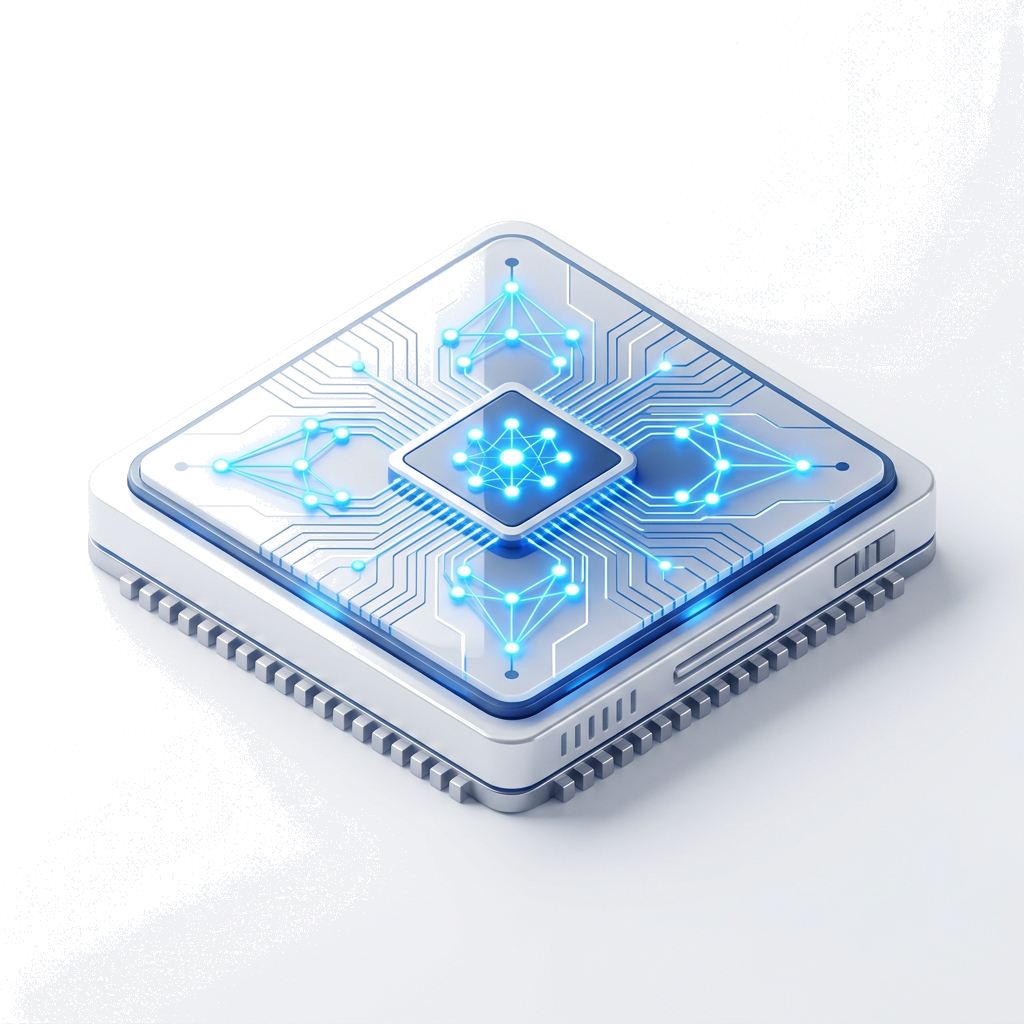
\includegraphics[width=0.65cm]{icons/llm_chip.png}};

%── (4) LOGITS ────────────────────────────────────────────────────────
\node[blk=Blue](LOG) at (0,-4.00)
  {Decision-Logit Extraction \;
   $\mathbf{z}_{0:N}\!\in\!\mathbb{R}^{(N+1)\times 2}$};

%── (5) REWARD ────────────────────────────────────────────────────────
\node[blk=Blue,minimum height=0.84cm](RW) at (0,-5.12)
  {Reward \& Conflict Estimation\\[1pt]
   {\footnotesize\normalfont\mdseries
    $r_i = \Delta_i - \Delta_{\mathrm{base}},\quad
     \sigma^2 = \mathrm{Var}(\Delta_{1:N})$}};

%── (6) DIAMOND ───────────────────────────────────────────────────────
\node[diamond,draw=Red,fill=Red!9,lw=1.0pt,
      minimum width=3.2cm,minimum height=1.04cm,
      text centered,font=\small\bfseries\sffamily,
      inner sep=0pt,text=Ink]
  (GT) at (0,-7.00){$\sigma^2 \!\ge\! \tau_c$?};

%── MPPI BLOCK (x=5.62) ────────────────────────────────────────────────
% Gear + label — anchor=south at y=-6.10
% panel.north ≈ -5.60 < RW.south=-5.54 (barely safe; use -6.14 for margin)
\node[font=\footnotesize\bfseries\sffamily,text=Red,anchor=south]
  (ML) at (5.62,-6.14) {%
  \raisebox{-0.06cm}{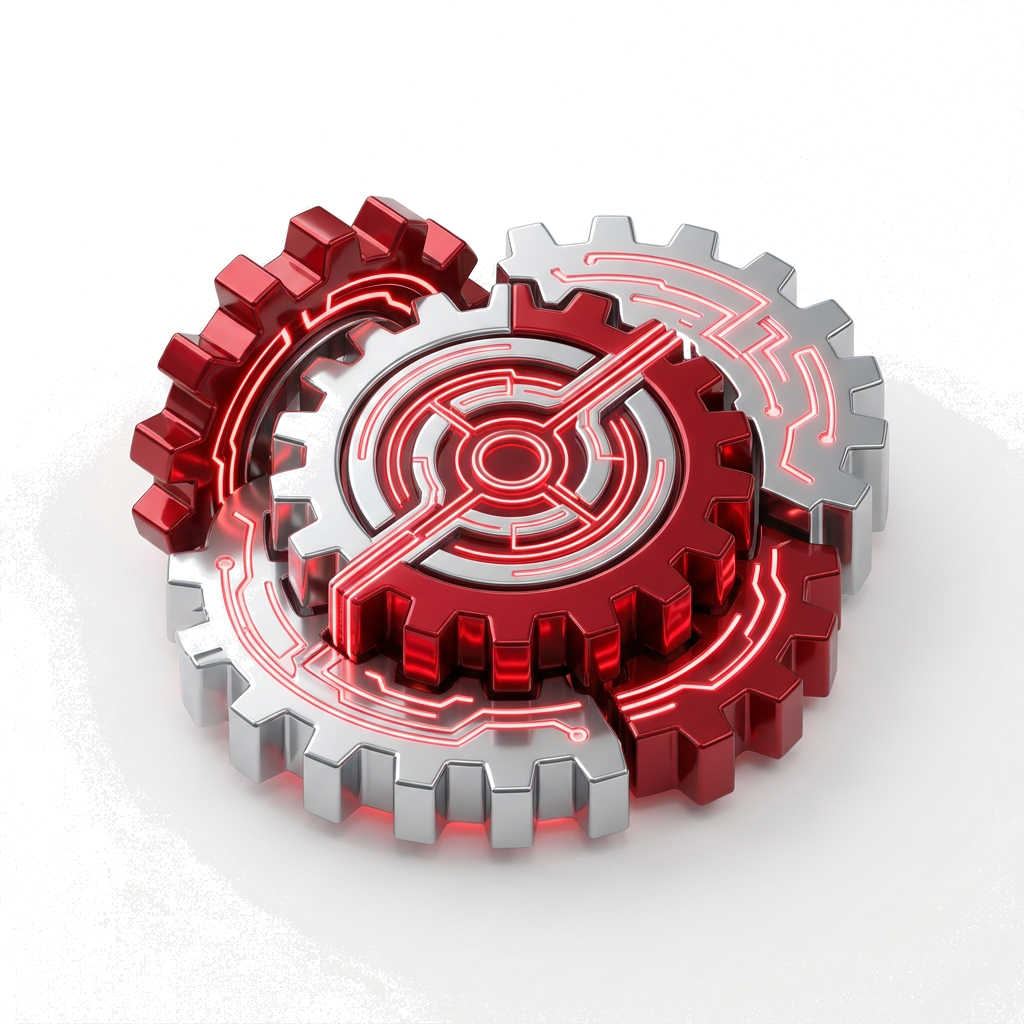
\includegraphics[width=0.30cm]{icons/mppi_gears.png}}%
  \enspace MPPI Solver};

\node[mppiblk](M1) at (5.62,-6.52){Sample $K$ perturbations $\epsilon_k$};
\node[mppiblk](M2) at (5.62,-7.20){Prospect-Theory Utility $v(\!\cdot\!)$};
\node[mppiblk](M3) at (5.62,-7.88){Cooperative Softmax $\to\!\delta^*$};

\draw[Ar](M1.south)--(M2.north);
\draw[Ar](M2.south)--(M3.north);

\begin{scope}[on background layer]
  \node[panel=Red,fit=(ML)(M1)(M2)(M3)](MB){};
\end{scope}

%── (7) AGGREGATION ───────────────────────────────────────────────────
\node[blk=Red,minimum height=0.72cm](AGG) at (0,-8.82)
  {Decision Aggregation \;
   $\delta_{\mathrm{opt}} = \delta_{\mathrm{cons}} + \delta^*$};

%── (8) DEBIASING ─────────────────────────────────────────────────────
\node[blk=Blue,minimum height=0.84cm](DEB) at (0,-9.94)
  {Two-Pass Positional Debiasing\\[1pt]
   {\footnotesize\normalfont\mdseries
    original $+$ L$\leftrightarrow$R swap $\;\to\;$ avg $\bar{p}_{\mathrm{pref}}$}};

%── (9) AMCE ──────────────────────────────────────────────────────────
\node[blk=Grn](AMC) at (0,-11.06)
  {AMCE Score \;
   $\hat{a}_c = \mathbb{E}_s\!\left[p_{\mathrm{spare\text{-}pref}}(s)\right]$};

%── (10) CULTURAL ALIGNMENT ───────────────────────────────────────────
\node[blk=Grn,minimum height=0.72cm](ALN) at (0,-12.08)
  {Cultural Alignment \;
   $\rho_c,\;\mathrm{JSD}(\hat{a}_c \!\parallel\! h_c),\; r_{\mathrm{Pearson}}$};

% Globe badge at NW corner of Cultural Alignment
\node[inner sep=0pt] at ($(ALN.west)+(0,0)$){
\includegraphics[width=0.65cm]{icons/culture_globe.png}};

%══════════════════════════════════════════════════════════════════════
%  ARROWS
%══════════════════════════════════════════════════════════════════════
\draw[A](IN.south)--(PB.north);
\draw[A](PB.south)--(LLM.north);
\draw[A](LLM.south)--(LOG.north);
\draw[A](LOG.south)--(RW.north);
\draw[A](RW.south)--(GT.north);

\draw[Ar](GT.east)
  -- node[above,font=\scriptsize\bfseries\sffamily,text=Red,
          inner sep=2pt,pos=0.50]{\textsc{yes}}
  ++(0.72,0) |- (M1.west);

\draw[Ar](M3.south)--++(0,-0.22)-|(AGG.east);

\draw[A](GT.south)
  -- node[right,font=\scriptsize\bfseries\sffamily,text=Ink!65,
          inner sep=3pt,pos=0.35]{\textsc{no}}
  (AGG.north);

\draw[A] (AGG.south)--(DEB.north);
\draw[Ag](DEB.south)--(AMC.north);
\draw[Ag](AMC.south)--(ALN.north);

%══════════════════════════════════════════════════════════════════════
%  GROUP PANELS
%══════════════════════════════════════════════════════════════════════
\begin{scope}[on background layer]
  \node[panel=Blue,fit=(PB)(LLM)(LOG),
    label={[font=\scriptsize\bfseries\sffamily,Blue,
            rotate=90,anchor=south,yshift=5pt]west:
            Multi-Agent Encoding}]{};
  \node[panel=Grn,fit=(AMC)(ALN),
    label={[font=\scriptsize\bfseries\sffamily,Grn,
            rotate=90,anchor=south,yshift=5pt]west:
            Evaluation}]{};
\end{scope}

\end{tikzpicture}
\end{document}
